\chapter{Page Tables and Memory Management}\label{ch:page-tables-and-memory-management}

\section{Memory Management Overview}\label{sec:3-memory-management-overview}

Memory management (Memory Management) refers to the operations of allocating and reclaiming physical
memory (Physical
Memory) and the virtual address
space (Virtual Address
Space, VAS). To guarantee the safety of memory management, support at the hardware level is necessary. The memory management of the RME operating system supports memory
protection unit (Memory
Protection Unit, MPU) environments and memory management
unit (Memory Management
Unit, MMU) environments, and they are abstracted into the same page table data structure. The terms used in this chapter are defined as follows:

\begin{xltabular}{\textwidth}{@{}>{\hsize=0.7749\hsize\raggedright\arraybackslash}X>{\hsize=1.2251\hsize\raggedright\arraybackslash}X@{}}
\caption{Page Directory Terminology Definitions}\label{tab:3-1-page-directory-terminology}\\
\toprule
Term & Definition\tabularnewline
\endfirsthead
\toprule
Term & Definition\tabularnewline
\midrule
\endhead
\bottomrule
\endlastfoot
Page table (Page Table, PT) &
Refers to the entire page table itself, including the top-level page directory and the page directories at each intermediate level; it is the general term for an address tree.\tabularnewline
Page directory (Page Directory, PD) &
Refers to one level of the page table, of which the topmost level is called the top-level page directory.\tabularnewline
Page entry (Page Entry, PE) &
Refers to an entry in the page directory table; it may point to a page, or it may point to the next-level page directory. Among these, the ones that point to a page are called page
terminal entries (Page
Terminal Entry, PTE), and those that point to a next-level page directory are called page
intermediate entries (Page
Intermediate Entry, PIE).\tabularnewline
\end{xltabular}
\nopagebreak[4]

\section{Page Table Operations and Structure}\label{sec:3-page-table-operations-and-structure}

A page table is a multi-level radix trie (Radix Trie/Radix
Tree) structure composed of a series of page directories. Each slot of a page directory is fixed to the length of one machine word. Each slot in a page directory can hold one of the following three kinds of data: the physical address of a lower-level page directory, the physical address and attributes of a page table entry, or an empty page table entry. If what is stored is the physical address of a lower-level page directory, then it means that a lower-level page directory exists here, and the mapping relationship of that part of the virtual address is to be determined by looking it up in that page directory; if what is stored is the physical address and attributes of a page table entry, then it means that a page table entry is mapped at this virtual address, and the access attributes of that page can be known; if what is stored is an empty page table entry, then it means that nothing is mapped at this virtual address. In RME, page tables must be constructed manually by the user, which is consistent with the solution approach of a series of microkernels such as Composite\hyperref[cite:3-1]{{[}1{]}}.

\subsection{Kernel Memory and User Memory}\label{subsec:3-kernel-memory-and-user-memory}

The system memory of RME is divided into two parts: one part is kernel memory, and one part is user memory. Unlike microkernels such as Composite and L4, in the RME system the kernel memory mapping is fully established at the very beginning\footnote{Static or semi-static allocation} and cannot be modified. This makes RME completely free of the need for a memory dynamic typing mechanism\footnote{This mechanism is adopted by systems such as Composite and seL4\hyperref[cite:3-1]{{[}1{]}}\hyperref[cite:3-3]{{[}3{]}}. In RME it can actually also be implemented by a trusted user-mode server}, and the memory management system is fully parallelizable, while at the same time completely eliminating the possibility of kernel memory content leakage. For MMU environments, when creating a top-level page directory, the system maps the kernel page directory created at boot time into the top-level page directory; for MPU environments, since kernel mode usually has access permission to the entire memory, we only need user pages in all page directories\footnote{Some architectures (such as Tricore) need to reserve one or more MPU register groups for kernel mode, but these pages are not reflected in the page table}.

At system boot, all user physical memory pages are added to the page table of the boot process (Init). After this addition is complete, generally the system is no longer allowed to create physical memory page frames out of thin air, unless a custom kernel call is used\footnote{See Section~\ref{sec:8-kernel-call-implementation-overview}}. When creating a new process, the page table entries of the new process's page table must be added from other processes. During the addition, the access attributes of this page can be specified, and the specified access attributes must be a subset of the access attributes of the parent page. In the RME system, the standard attributes for page access are as follows:

\begin{xltabular}{\textwidth}{@{}>{\hsize=0.5857\hsize\raggedright\arraybackslash}X>{\hsize=0.7809\hsize\raggedright\arraybackslash}X>{\hsize=1.6334\hsize\raggedright\arraybackslash}X@{}}
\caption{Standard Page Access Attributes}\label{tab:3-2-standard-page-access-attributes}\\
\toprule
Name & Identifier & Meaning\tabularnewline
\endfirsthead
\toprule
Name & Identifier & Meaning\tabularnewline
\midrule
\endhead
\bottomrule
\endlastfoot
Readable & RME\_PGT\_READ & This page is readable.\tabularnewline
Writable & RME\_PGT\_WRITE & This page is writable.\tabularnewline
Executable & RME\_PGT\_EXECUTE &
This page can be executed as code.\tabularnewline
Cacheable & RME\_PGT\_CACHE & The contents of this page can be cached.\tabularnewline
Bufferable & RME\_PGT\_BUFFER & Writes to this page can be buffered.\tabularnewline
Static & RME\_PGT\_STATIC &
This page is a static page that is always mapped. This means that in MPU environments or in MMU environments with manual TLB updates, this page is always mapped, rather than being mapped only when a page fault occurs.\tabularnewline
\end{xltabular}
\nopagebreak[4]

It is worth noting that on some architectures, some of the above bits may not all be meaningful. For example, for the vast majority of MMU environments that automatically update the translation look-aside
buffer (Trans
Look-aside
Buffer, TLB), the static attribute is meaningless; for some architectures, read and write are implemented together, so there is no separate read and write control.

To enable user mode to manage kernel memory when creating kernel objects, the kernel objects in the system are managed using a kernel object registry. The kernel object registry is a bitmap that stores the occupancy of virtual addresses by kernel objects. This bitmap guarantees that two kernel objects cannot exist on the same segment of kernel virtual address at the same time.

To prevent certain system components that have the right to create kernel objects from creating a large number of kernel objects when they fail or are compromised, thereby exhausting kernel memory and launching a denial-of-service (Denial
of
Service, DoS) attack, a kernel memory capability is therefore introduced to manage kernel memory. The concept of the kernel memory capability draws on the kernel object factory (Factory) of Fiasco.OC\hyperref[cite:3-4]{{[}4{]}}. When creating any kernel object, a kernel memory capability is required; this kernel memory capability indicates the kernel virtual memory address range permitted for use in creating kernel objects, as well as which objects are permitted to be created on this memory. Only when the kernel object being created falls entirely within this range, and the flag bits of the kernel memory capability permit the creation of this kind of object, can the creation operation continue; otherwise an error is returned, thereby restricting certain infected malicious kernel components from launching denial-of-service attacks.

\subsection{Page Directory Attributes}\label{subsec:3-page-directory-attributes}

In the RME operating system, a page directory has four attributes. These four attributes uniquely determine the state of the page directory. We introduce these four attributes separately below.

\subsubsection{Mapping Base Address}\label{subsubsec:3-mapping-base-address}

The mapping base address refers to the virtual address at which this level of page directory begins mapping. The physical memory of the first slot of this page directory, or the base address of the second-level page table it maps, is this virtual address. When we attempt to map a lower-level page directory to a certain position of a certain higher-level page directory, we may need to check whether the lower-level virtual address matches the higher-level virtual address, so as to determine whether the mapping can be performed. Of course, this check is necessary only in systems that use an MPU. In systems that use an MMU, since a page directory is often mapped into different positions of different page directories, this check can be configured not to be performed; in that case the mapping base address item is invalid, and the path-compressed page table (Path-Compressed
Page
Table, PCPT) format also cannot be used\footnote{MMU systems generally do not support this format either}. For the differences regarding the path-compressed page table format, MPU systems and MMU systems, please see the following chapters.

\subsubsection{Top-Level Page Directory Flag}\label{subsubsec:3-top-level-page-directory-flag}

Indicates that this page directory is the topmost page directory. Only the topmost page directory can be used to create a process.

\subsubsection{Page Directory Size Order}\label{subsubsec:3-page-directory-size-order}

The page directory size order determines the size of the virtual address represented by each slot of the page directory. If the size order of a page directory is 12, then it means that each slot in this page directory corresponds to a page of size 2\textsuperscript{12}=4096 bytes.

\subsubsection{Page Directory Number Order}\label{subsubsec:3-page-directory-number-order}

The page directory number order determines the number of slots in the page directory. If the number order of a page directory is 10, then it means that this page directory has a total of 2\textsuperscript{10}=1024 slots.

\subsection{Basic Page Directory Operations}\label{subsec:3-basic-page-directory-operations}

There are altogether six basic operations on a page directory, as follows:

\begin{xltabular}{\textwidth}{@{}>{\hsize=0.8417\hsize\raggedright\arraybackslash}X>{\hsize=1.1583\hsize\raggedright\arraybackslash}X@{}}
\caption{Basic Page Directory Operations}\label{tab:3-3-basic-page-directory-operations}\\
\toprule
Operation & Meaning\tabularnewline
\endfirsthead
\toprule
Operation & Meaning\tabularnewline
\midrule
\endhead
\bottomrule
\endlastfoot
Create page directory (Create) & Create a new empty page directory.\tabularnewline
Delete page directory (Delete) & Delete a page directory.\tabularnewline
Map memory page (Add) &
Add a physical memory page at a certain virtual address of the page directory.\tabularnewline
Remove memory page (Remove) &
Delete a physical memory page at a certain virtual address of the page directory.\tabularnewline
Construct page directory (Construct) &
Add a child page directory at a certain virtual address of a parent page directory.\tabularnewline
Destruct page directory (Destruct) &
Delete a child page directory mapped at a certain virtual address of the parent page directory.\tabularnewline
\end{xltabular}
\nopagebreak[4]

The implementations of these six operations on MPU and MMU are very different, and they also have different restrictions. Please refer to the explanations in the following two sections to understand the specific differences.

\subsection{Implementation of a Normal Multi-Level Page Table Under the Memory Management Unit}\label{subsec:3-normal-multilevel-page-table-under-mmu}

For the memory management unit, the implementation of a page directory is very simple: it is just a simple linear table. For example, for the x86-64 page table, its first-level page directory (PML4) has fixed 512 slots, each slot representing 2\textsuperscript{39} bytes; the second-level page directory (PDP) also has fixed 512 slots, each slot representing 2\textsuperscript{30} bytes; the third-level page directory (PGD) also has fixed 512 slots, each slot representing 2\textsuperscript{21} bytes; and the fourth-level page directory (PTE) also has fixed 512 slots, each slot representing 2\textsuperscript{12} bytes. The radix tree formed by these four levels of page directories is the entire page table, as shown in the figure below. Among them, blue slots represent entries pointing to child page directories, while gray slots represent mapped pages. In addition, the memory base addresses of these page directories should all be aligned to 4kB, so that they each occupy exactly one page.

\begin{figure}[htbp]
    \centering
    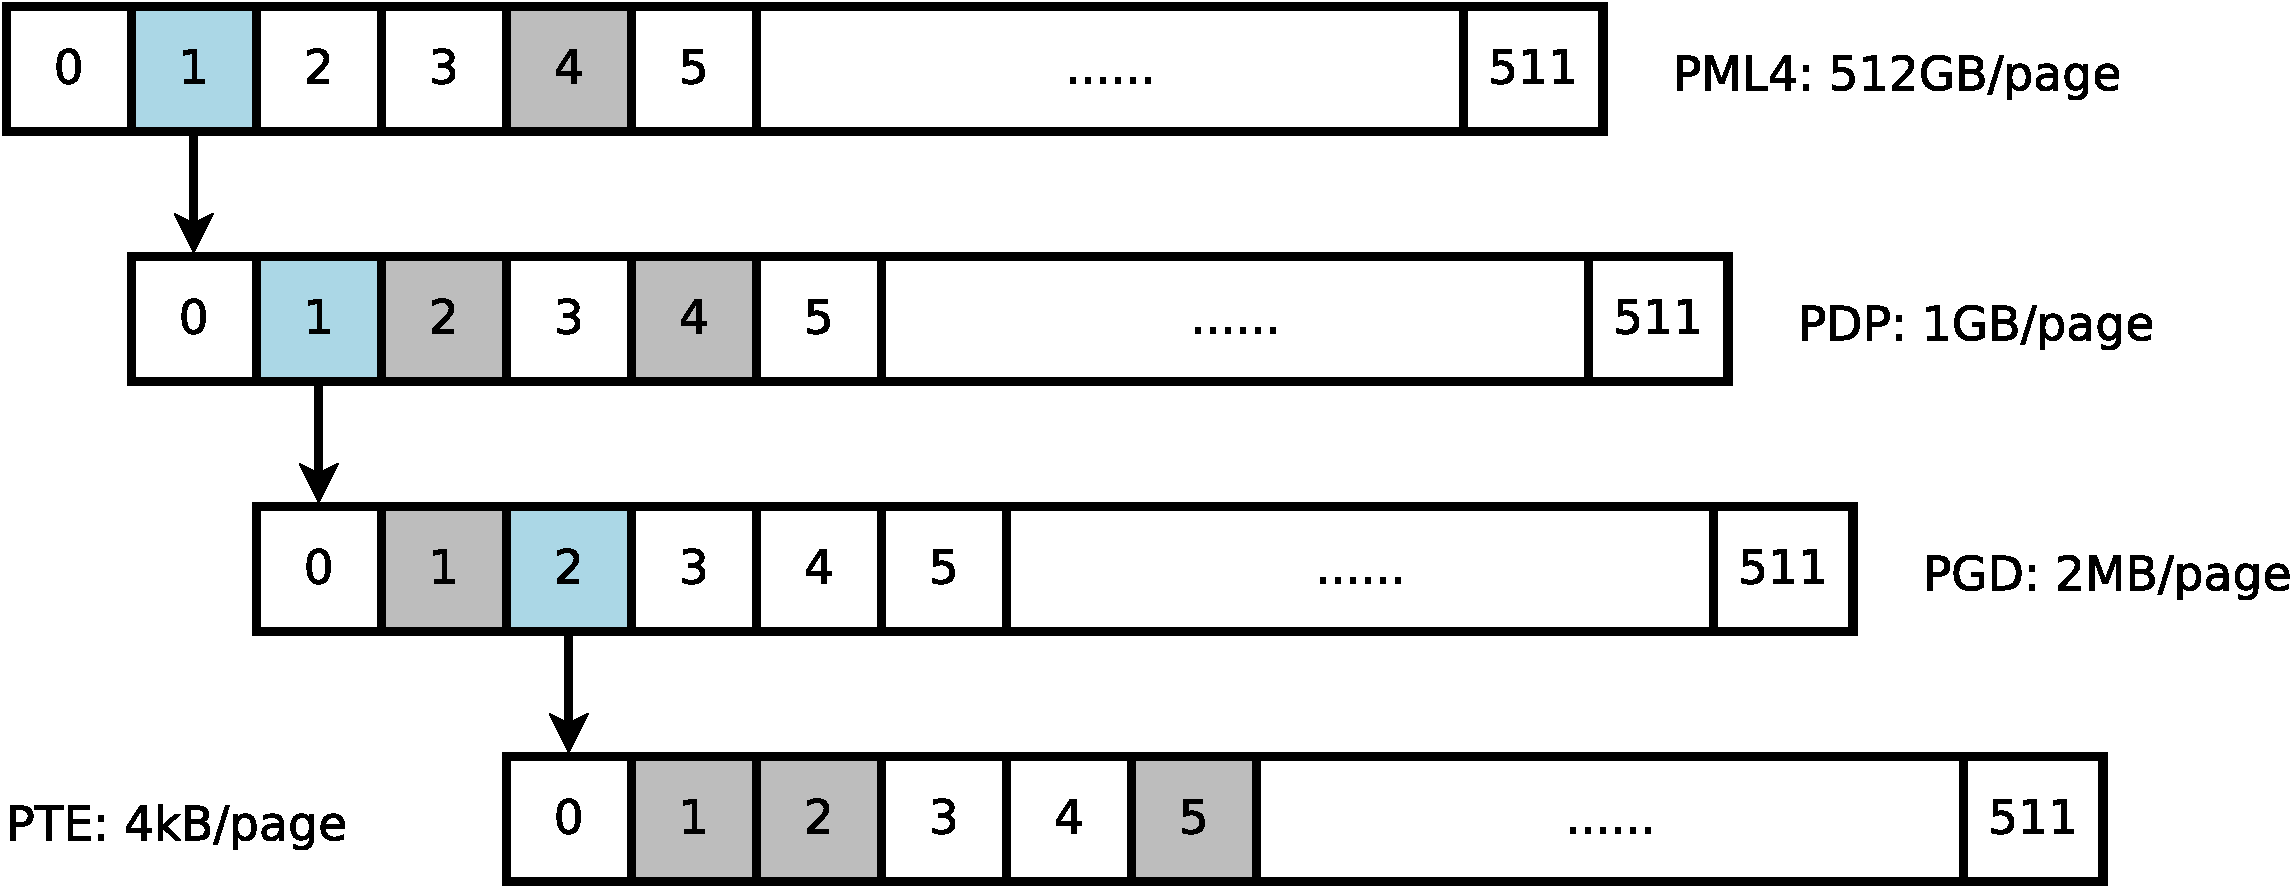
\includegraphics[width=0.72\textwidth]{Figure/image8.pdf}
    \caption{An Example of a Normal Multi-Level Page Table}
    \label{fig:3-1-normal-multilevel-page-table-example}
\end{figure}

In addition, if a page directory is allowed to be constructed into any virtual address slot of a higher-level page directory\footnote{As long as the size order and number order are appropriate}, then we can configure the kernel not to check whether the starting virtual address is appropriate. In this case, we are using a normal multi-level page table, and there is no need to implement path compression.

Since the processor has hardware that handles page tables directly, we do not need to generate page table metadata specifically for the processor. However, it should be noted that when the page table creation function is called, the created page table should conform to the requirements of the hardware page table lookup mechanism. For those MMUs whose TLB is filled purely by software, there is no such requirement; tree structures that logically conform to the form of a page table can be created at will, and these MMUs can also be regarded as region-based MMUs and handled in the way described in \ref{subsec:3-path-compressed-page-table-under-mpu}.

\needspace{16\baselineskip}
Some common features of MMUs are as follows:

\begin{xltabular}{\textwidth}{@{}>{\hsize=0.8979\hsize\raggedright\arraybackslash}X>{\hsize=0.6440\hsize\raggedright\arraybackslash}X>{\hsize=1.4399\hsize\raggedright\arraybackslash}X>{\hsize=1.0182\hsize\raggedright\arraybackslash}X@{}}
\caption{Features of Common MMUs}\label{tab:3-4-common-mmu-features}\\
\toprule
Processor & Page Table Levels & Page Size & Other Features\tabularnewline
\endfirsthead
\toprule
Processor & Page Table Levels & Page Size & Other Features\tabularnewline
\midrule
\endhead
\bottomrule
\endlastfoot
ARM926EJ-S & 2 or 3 levels & 1MB, 64kB, 4kB, 1kB &
Manual locking of some TLB entries\tabularnewline
x86-64 (AMD64) & 3 levels & 1GB, 2MB, 4kB &
Additional segment-based memory management unit\tabularnewline
Itanium (IA-64) & 4 levels & 256MB, 16MB, 4MB, 1MB, 256kB, 64kB, 8kB, 4kB &
Partially manually fillable TLB\tabularnewline
e200 (PowerPC) & Not applicable & All powers of 2 from 1kB to 4GB &
Purely software-filled TLB\tabularnewline
ARMv7-A (32-bit) & 2 or 3 levels & 4kB, 64kB, 1MB, 16MB &
Manual locking of some TLB entries\tabularnewline
ARMv8-M (64-bit) & 3 or 4 levels & 4kB, 16kB, 64kB &
Optional stage-2 translation under virtualization\tabularnewline
MIPS64 & Not applicable & All powers of 4 from 1kB to 256MB &
Purely software-filled TLB\tabularnewline
TMS320C66X & Not applicable & All powers of 2 from 4kB to 4GB &
Purely software-filled TLB\tabularnewline
\end{xltabular}
\nopagebreak[4]

\subsection{Implementation of a Path-Compressed Page Table Under the Memory Protection Unit}\label{subsec:3-path-compressed-page-table-under-mpu}

Under the memory protection unit\footnote{Or a manually filled, region-based memory management unit; the same below}, the processor often cannot directly recognize multi-level page tables. This obliges us to generate MPU metadata from the page table, to be used to set up the MPU efficiently at process switch. Moreover, in MPU environments there are also the following characteristics:

\begin{enumerate}
\def\labelenumi{\arabic{enumi}.}
\item
  The number of MPU regions is often limited; for example, ARMv7-M has at most 16 regions, and each region can in turn be divided into 8 subregions. Therefore, in one process we can allow at most 128 regions to be mapped simultaneously, and these regions must also satisfy a series of stringent conditions such as address alignment. Therefore, we can consider dividing pages into two classes: one class is static pages, which are always mapped and can be used by applications requiring predictability; the maximum number of static pages is exactly the maximum number of MPU regions allowed by the processor. The other class is dynamic pages, which are mapped only when in use and are not guaranteed to be mapped at all times; the maximum number of dynamic pages is unlimited. If a dynamic page that is not currently mapped is accessed, the processor enters the page fault exception, and we then manually look up the page table to add this dynamic page to the MPU metadata; at this point, if there are not enough MPU regions, other dynamic pages may be replaced\hyperref[cite:3-2]{{[}2{]}}.
\item
  In a page table, often only one or two entries exist. For microcontrollers that use an MPU, maintaining the existence of multi-level page tables is an unnecessary waste of resources, so a way should be found to compress the page table. Compared with an ordinary page table, in a compressed page table the number of address bits translated by different page intermediate entries of the same page directory can be different. For example, at a certain virtual address there is a very small page that we need to add to the access range. For an ordinary page table, we need multiple levels of intermediate page directories, and then at the last-level page directory we add this page. For a compressed page table, however, a single level of page directory is enough to address this page. We can state the base address, number order and size order of this page directory, and then directly construct it into the upper-level page directory. Of course, in this case we require that the virtual address range represented by this level of page table fall within the virtual address range permitted by the corresponding page table entry of the upper-level page directory. There is one exception to the above situation: when the architecture actually has a region-based MMU unit, we usually do not use a path-compressed page table.
\item
  The MPU cannot perform physical-address-to-virtual-address translation. Therefore, the virtual address is always equal to the physical address. This obliges us to check, when mapping a page, whether the mapping address of the page is equal to the physical address.
\item
  Since we need MPU metadata to speed up MPU filling, when we modify any level of page directory we must maintain consistency between the metadata and the page table. It is also possible not to maintain this consistency, but if we do so, we can only update the metadata through page faults. And updating the metadata through page faults is not always possible: some architectures do not provide key information such as the faulting address in some or all cases. For detailed information on this approach, please refer to \ref{subsubsec:3-update-mpu-metadata-on-page-fault}.

  An example of a path-compressed page table on ARMv7-M is shown in the figure below. Green slots represent path-compressed entries pointing to child page directories, blue slots represent non-path-compressed entries pointing to child page directories, and gray slots represent mapped pages. The hexadecimal numbers in front of the page tables at each level represent the starting mapping address of that page table.

\begin{figure}[htbp]
    \centering
    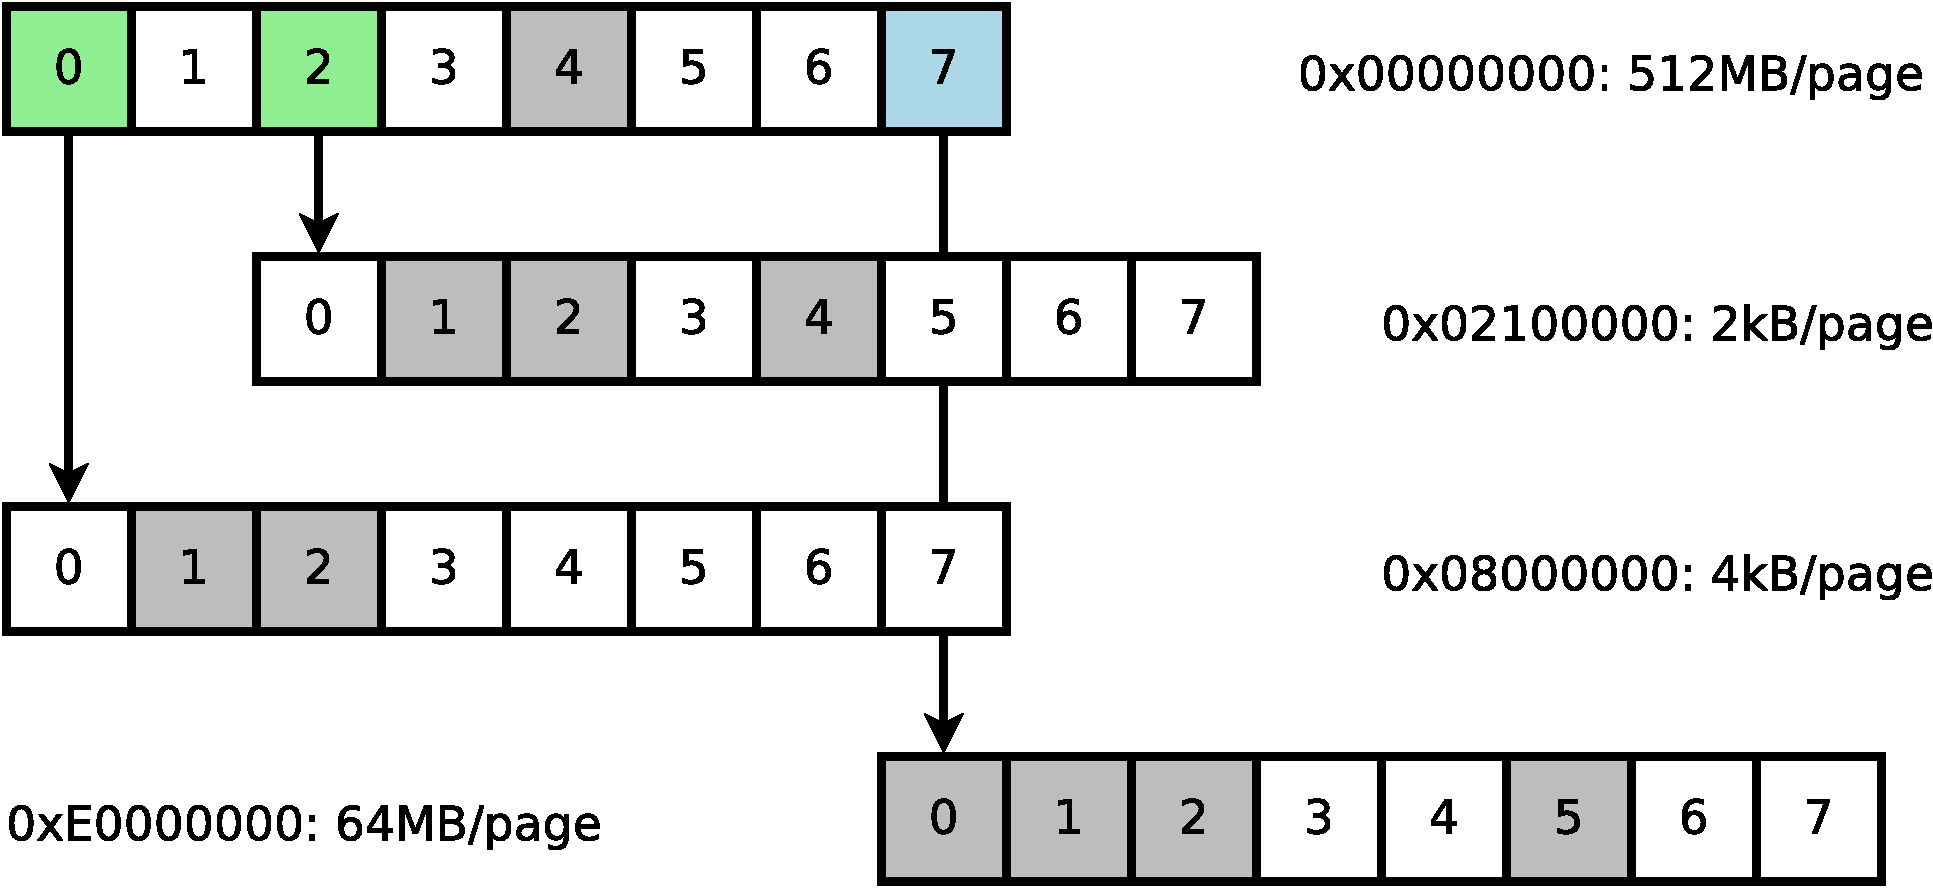
\includegraphics[width=0.72\textwidth]{Figure/image9.pdf}
    \caption{An Example of a Path-Compressed Page Table}
    \label{fig:3-2-path-compressed-page-table-example}
\end{figure}

  Some common features of MPUs are as follows:
\end{enumerate}

\begin{xltabular}{\textwidth}{@{}>{\hsize=1.0901\hsize\raggedright\arraybackslash}X>{\hsize=0.8740\hsize\raggedright\arraybackslash}X>{\hsize=1.1654\hsize\raggedright\arraybackslash}X>{\hsize=0.8740\hsize\raggedright\arraybackslash}X>{\hsize=0.9663\hsize\raggedright\arraybackslash}X>{\hsize=1.0301\hsize\raggedright\arraybackslash}X@{}}
\caption{Features of Common MPUs}\label{tab:3-5-common-mpu-features}\\
\toprule
Processor & Number of Regions & Region Organization & Size Range & Alignment Requirement &
Other Features\tabularnewline
\endfirsthead
\toprule
Processor & Number of Regions & Region Organization & Size Range & Alignment Requirement &
Other Features\tabularnewline
\midrule
\endhead
\bottomrule
\endlastfoot
ARM v6-M & 0 to 16 & Unified organization & 128B-4GB & Aligned to size &
8 subregions\tabularnewline
ARM v7-M & 0 to 16 & Unified organization & 128B-4GB & Aligned to size &
8 subregions\tabularnewline
ARM v8-M & 0 to 16 & Unified organization & 128B-4GB & None & None\tabularnewline
Tensilica L106 & 16 or 32 & Unified organization & 4kB-1GB & None & None\tabularnewline
MIPS M14k & 1 to 16 & Unified organization & Arbitrary & None & Can be locked as read-only\tabularnewline
PowerPC e200z4 & 32 & 16 each for code/data & Arbitrary & None & None\tabularnewline
AVR32 & 8 & Unified organization & 4kB-4GB & Aligned to size &
16 subregions\tabularnewline
MSP430FRXX & 3 & Unified organization & Arbitrary & None & Three-segment segmented\tabularnewline
Coldfire-MCF & 4 & 2 each for code/data & 16MB-4GB & Aligned to size &
None\tabularnewline
RISC-V & 0 to 16 & Unified organization & 4B-4GB & Aligned to size &
Can also be aligned to words\tabularnewline
\end{xltabular}
\nopagebreak[4]

In summary, for the implementation of page tables under an MPU, the following two forms are common:

\subsubsection{Immediately Update MPU Metadata When Updating the Page Table}\label{subsubsec:3-update-mpu-metadata-immediately}

This approach places the MPU metadata only in the top-level page directory, and requires construction to start from the top level. If any level of page directory does not have a top-level page directory and is not itself a top-level page directory, then no child page directory can be constructed into this page directory. In addition, any two page tables cannot share a page directory or a page directory tree. The restrictions of this implementation are as follows:

\begin{xltabular}{\textwidth}{@{}>{\hsize=0.5941\hsize\raggedright\arraybackslash}X>{\hsize=1.4059\hsize\raggedright\arraybackslash}X@{}}
\caption{Restrictions of Immediately Updating MPU Metadata When Updating the Page Table}\label{tab:3-6-immediate-mpu-metadata-update-constraints}\\
\toprule
Operation & Restriction or Disadvantage\tabularnewline
\endfirsthead
\toprule
Operation & Restriction or Disadvantage\tabularnewline
\midrule
\endhead
\bottomrule
\endlastfoot
Create process & No restriction.\tabularnewline
Change process page table & No restriction.\tabularnewline
Switch process & No restriction; simply use the MPU metadata in the top-level page directory.\tabularnewline
Create page directory & No restriction.\tabularnewline
Delete page directory & No restriction.\tabularnewline
Map memory page &
If it has a top-level page directory itself, update the MPU metadata of the top-level page directory.\tabularnewline
Remove memory page &
If it has a top-level page directory itself, update the MPU metadata of the top-level page directory.\tabularnewline
Construct page directory &
The parent page directory must itself have a top-level page directory, or must itself be a top-level page directory; the child page directory must not have a top-level page directory, and must not itself be a top-level page directory\footnote{And it is impossible for it to have child page directories either}. Add the mapped pages of the child page directory to the MPU metadata of the top-level page directory.\tabularnewline
Destruct page directory &
The child page directory must have a top-level page directory, and must not contain any child page directories\footnote{Its child page directories must be destructed from this page directory in advance}. Remove the mapped pages of the child page directory from the MPU metadata of the top-level page directory.\tabularnewline
Memory consumption & MPU metadata exists only in the top-level page directory.\tabularnewline
\end{xltabular}
\nopagebreak[4]

This implementation is the recommended implementation on single-core systems. This implementation maximizes the efficiency of MPU-based microcontrollers, so that we can often use pre-generated MPU metadata to set the MPU registers in bulk, with only some loss of infrequently used functionality. When the page table structure changes, its MPU metadata is also always updated immediately, so there is no potential real-time problem caused by page faults.

On some architectures, it is sometimes\footnote{Such as ARMv7-M: the page fault generated during hardware push and pop does not provide the faulting address, so dynamic pages cannot be used for the stack} or always\footnote{Such as ARMv6-M: because it is extremely streamlined, it does not provide any exception handling information under any circumstances, so it does not support dynamic pages at all} impossible to determine the faulting address in a page fault, and impossible to dynamically map pages based on the address. Because of the lack of exception handling information, such architectures do not support dynamic pages in some or all cases.

\subsubsection{Update MPU Metadata on Page Fault}\label{subsubsec:3-update-mpu-metadata-on-page-fault}

This approach treats the MPU metadata placed at the top-level page directory as a software-filled TLB, using a software page table walk algorithm in the memory protection interrupt to fill it on every miss. It does not attempt to generate the MPU metadata corresponding to the entire page table at once, but instead chooses to generate it gradually. Whenever the page table structure changes or the page mapping changes, all MPU metadata is cleared, which is equivalent to a TLB flush under the MMU architecture. This approach also supports static pages and dynamic pages, and a static page incurs a page fault only on its first access, while subsequent accesses can guarantee real-time behavior.

\begin{xltabular}{\textwidth}{@{}>{\hsize=0.8054\hsize\raggedright\arraybackslash}X>{\hsize=1.1946\hsize\raggedright\arraybackslash}X@{}}
\caption{Restrictions of Updating MPU Metadata on Page Fault}\label{tab:3-7-page-fault-mpu-metadata-update-constraints}\\
\toprule
Operation & Restriction or Disadvantage\tabularnewline
\endfirsthead
\toprule
Operation & Restriction or Disadvantage\tabularnewline
\midrule
\endhead
\bottomrule
\endlastfoot
Create process & No restriction.\tabularnewline
Change process page table & Clear the MPU metadata, ready for rebuilding.\tabularnewline
Switch process & No restriction.\tabularnewline
Create page directory & No restriction.\tabularnewline
Delete page directory & No restriction.\tabularnewline
Map memory page & No restriction.\tabularnewline
Remove memory page & Clear the MPU metadata, ready for rebuilding.\tabularnewline
Construct page directory & No restriction.\tabularnewline
Destruct page directory & Clear the MPU metadata, ready for rebuilding.\tabularnewline
Memory consumption & MPU metadata exists only in the top-level page directory.\tabularnewline
\end{xltabular}
\nopagebreak[4]

This implementation preserves the greatest compatibility with MMU systems, and is also the recommended implementation approach on multi-core MPU architectures. It imposes no requirement on the construction order of the page table, is also convenient for operations in multi-core environments, and multiple page tables can share a part in any manner, but its real-time performance is slightly worse than the scheme listed in \ref{subsubsec:3-update-mpu-metadata-immediately}.

\needspace{30\baselineskip}
\section{Page Table Function List}\label{sec:3-page-table-function-list}
\nopagebreak[4]

\needspace{20\baselineskip}
The kernel functions related to page tables are as follows:

\begin{xltabular}{\textwidth}{@{}>{\hsize=1.1605\hsize\raggedright\arraybackslash}X>{\hsize=0.8843\hsize\raggedright\arraybackslash}X>{\hsize=0.9552\hsize\raggedright\arraybackslash}X@{}}
\caption{Page Table Related Kernel Functions}\label{tab:3-8-page-table-related-kernel-functions}\\
\toprule
Call Number & Type & Purpose\tabularnewline
\endfirsthead
\toprule
Call Number & Type & Purpose\tabularnewline
\midrule
\endhead
\bottomrule
\endlastfoot
RME\_SVC\_PGT\_CRT & System call & Create page directory\tabularnewline
RME\_SVC\_PGT\_DEL & System call & Delete page directory\tabularnewline
RME\_SVC\_PGT\_ADD & System call & Map memory page\tabularnewline
RME\_SVC\_PGT\_REM & System call & Remove memory page\tabularnewline
RME\_SVC\_PGT\_CON & System call & Construct page directory\tabularnewline
RME\_SVC\_PGT\_DES & System call & Destruct page directory\tabularnewline
\end{xltabular}
\nopagebreak[4]

The operation flags of a page table capability are as follows:

\begin{xltabular}{\textwidth}{@{}>{\hsize=1.1000\hsize\raggedright\arraybackslash}X>{\hsize=0.6199\hsize\raggedright\arraybackslash}X>{\hsize=1.2801\hsize\raggedright\arraybackslash}X@{}}
\caption{Page Table Operation Flags}\label{tab:3-9-page-table-operation-flags}\\
\toprule
Flag & Bit & Purpose\tabularnewline
\endfirsthead
\toprule
Flag & Bit & Purpose\tabularnewline
\midrule
\endhead
\bottomrule
\endlastfoot
RME\_PGT\_FLAG\_ADD\_SRC & {[}0{]} &
Allows this page directory to act as the source directory in page frame passing.\tabularnewline
RME\_PGT\_FLAG\_ADD\_DST & {[}1{]} &
Allows this page directory to act as the destination directory in capability delegation.\tabularnewline
RME\_PGT\_FLAG\_REM & {[}2{]} &
Allows removing page frames in this page directory.\tabularnewline
RME\_PGT\_FLAG\_CHILD & {[}3{]} &
Allows this page directory to act as a child page directory in page table construction or destruction.\tabularnewline
RME\_PGT\_FLAG\_CON\_PARENT & {[}4{]} &
Allows this page directory to act as a parent page directory in page table construction.\tabularnewline
RME\_PGT\_FLAG\_DES\_PARENT & {[}5{]} &
Allows this page directory to act as a parent page directory in page table destruction.\tabularnewline
RME\_PGT\_FLAG\_PRC\_CRT & {[}6{]} &
Allows this page table to be used as the process page table when creating a process.\tabularnewline
RME\_PGT\_FLAG\_PRC\_PGT & {[}7{]} &
Allows this page table to be used to replace the page table of a process.\tabularnewline
Other bits & Bit field & Operation range attributes.\tabularnewline
\end{xltabular}
\nopagebreak[4]

Regarding bit {[}6{]} and bit {[}7{]} in the above table, please refer to \ref{subsec:4-create-a-process} and \ref{subsec:4-change-process-capability-table}. When filling in operation flags in the page-table-related kernel functions, the RME\_PGT\_FLAG(HIGH,LOW,FLAG) macro must be used for filling, where HIGH is the upper limit of the operation position Pos, and LOW is the lower limit of the operation position Pos; the closed interval formed by [HIGH, LOW] is the allowed range of Pos. FLAG consists of the respective allowed operation flags in bits {[}7:0{]}.

\needspace{14\baselineskip}
\subsection{Creating a Page Directory}\label{subsec:3-create-page-directory}

\needspace{16\baselineskip}
This operation creates a page directory and places its capability into an existing capability table. The page directory creation operation requires the following parameters:

\begin{xltabular}{\textwidth}{@{}>{\hsize=0.7362\hsize\raggedright\arraybackslash}X>{\hsize=0.6815\hsize\raggedright\arraybackslash}X>{\hsize=0.6815\hsize\raggedright\arraybackslash}X>{\hsize=1.9007\hsize\raggedright\arraybackslash}X@{}}
\caption{Parameters Required for Creating a Page Directory}\label{tab:3-10-create-page-directory-parameters}\\
\toprule
Parameter Name & Type & Field & Description\tabularnewline
\endfirsthead
\toprule
Parameter Name & Type & Field & Description\tabularnewline
\midrule
\endhead
\bottomrule
\endlastfoot
Svc\_Num & ptr\_t & N.Q0 & Must be RME\_SVC\_PGT\_CRT.\tabularnewline
Cap\_Cpt & cid\_t & C &
A capability number corresponding to a capability table capability that must have the RME\_CPT\_FLAG\_CRT attribute; the capability corresponding to this capability number points to the capability table that is to receive the capability of this newly created page directory. This capability number may be a one-level or two-level lookup encoding.\tabularnewline
Cap\_Kom & cid\_t & P1.D1 &
A kernel memory capability number; the kernel memory range it identifies must be able to hold the entire page directory, and it must have the RME\_KOM\_FLAG\_PGT attribute. This capability number may be a one-level or two-level lookup encoding.\tabularnewline
Cap\_Pgt & cid\_t & P1.Q1 &
A capability number corresponding to a certain position in the capability table that receives the capability of this newly created page directory. The capability corresponding to this capability number must be empty. This capability number can only be a one-level lookup encoding.\tabularnewline
Raddr & ptr\_t & P2 &
The kernel relative starting virtual address to be used by the newly created page directory. This address is relative to the starting virtual address of the kernel capability corresponding to Cap\_Kom.\tabularnewline
Base & ptr\_t & P3 &
The mapping base address of the newly created page directory; the last bit is the top-level flag, see below.\tabularnewline
Is\_Top & ptr\_t & P3{[}0{]} &
Whether this page directory is a top-level page directory. ``1'' means that this page directory is top-level.\tabularnewline
Size\_Order & ptr\_t & P1.Q0 &
The size order of this page directory\footnote{Refers to the memory page size represented by each page table entry}.\tabularnewline
Num\_Order & ptr\_t & N.Q1 & The number order of this page directory.\tabularnewline
\end{xltabular}
\nopagebreak[4]

\needspace{16\baselineskip}
The possible return values of this operation are as follows:

\begin{xltabular}{\textwidth}{@{}>{\hsize=0.8188\hsize\raggedright\arraybackslash}X>{\hsize=1.1812\hsize\raggedright\arraybackslash}X@{}}
\caption{Possible Return Values for Creating a Page Directory}\label{tab:3-11-create-page-directory-return-values}\\
\toprule
Return Value & Meaning\tabularnewline
\endfirsthead
\toprule
Return Value & Meaning\tabularnewline
\midrule
\endhead
\bottomrule
\endlastfoot
    0 & The operation succeeded.\tabularnewline
    RME\_ERR\_CPT\_RANGE & The one-level/two-level lookup of Cap\_Cpt is out of range.\tabularnewline
    RME\_ERR\_CPT\_RANGE & The one-level/two-level lookup of Cap\_Kom is out of range.\tabularnewline
    RME\_ERR\_CPT\_RANGE & The one-level lookup of Cap\_Pgt is out of range.\tabularnewline
    RME\_ERR\_CPT\_FROZEN & The capability of the one-level/two-level lookup of Cap\_Cpt has been frozen.\tabularnewline
    RME\_ERR\_CPT\_FROZEN & The capability of the one-level/two-level lookup of Cap\_Kom has been frozen.\tabularnewline
    RME\_ERR\_CPT\_FROZEN & Cap\_Pgt is frozen, or another core is creating a capability at that location.\tabularnewline
    RME\_ERR\_CPT\_TYPE & Cap\_Cpt is not a capability table capability.\tabularnewline
    RME\_ERR\_CPT\_TYPE & Cap\_Kom is not a kernel memory capability.\tabularnewline
    RME\_ERR\_CPT\_FLAG & Cap\_Cpt has no RME\_CPT\_FLAG\_CRT attribute.\tabularnewline
    RME\_ERR\_CPT\_FLAG & Cap\_Kom has no RME\_KOM\_FLAG\_PGT attribute, or the range is incorrect.\tabularnewline
    RME\_ERR\_CPT\_EXIST & Cap\_Pgt is not an empty capability.\tabularnewline
    RME\_ERR\_CPT\_KOT & Allocation of kernel memory failed.\tabularnewline
    RME\_ERR\_PGT\_HW & Underlying hardware restriction; creating such a page directory is not allowed.\tabularnewline
\end{xltabular}
\nopagebreak[4]

\needspace{30\baselineskip}
\subsection{Page Directory Deletion}\label{subsec:3-delete-page-directory}
\nopagebreak[4]

This operation deletes a page directory. The page directory being deleted must not contain child page directories. Deleting a page directory requires the following parameters:

\begin{xltabular}{\textwidth}{@{}>{\hsize=0.6910\hsize\raggedright\arraybackslash}X>{\hsize=0.6910\hsize\raggedright\arraybackslash}X>{\hsize=0.6910\hsize\raggedright\arraybackslash}X>{\hsize=1.9271\hsize\raggedright\arraybackslash}X@{}}
\caption{Parameters Needed for Page Directory Deletion}\label{tab:3-12-delete-page-directory-parameters}\\
\toprule
Parameter Name & Type & Domain & Description\tabularnewline
\endfirsthead
\toprule
Parameter Name & Type & Domain & Description\tabularnewline
\midrule
\endhead
\bottomrule
\endlastfoot
Svc\_Num & ptr\_t & N & Must be RME\_SVC\_PGT\_DEL.\tabularnewline
Cap\_Cpt & cid\_t & C &
A capability number corresponding to a capability table capability that must have the RME\_CPT\_FLAG\_DEL attribute; the capability corresponding to this capability number points to the capability table containing the page directory capability being deleted. This capability number can be a one-level or two-level lookup encoding.\tabularnewline
Cap\_Pgt & cid\_t & P1 &
A capability number corresponding to the page directory capability to be deleted. The capability corresponding to this capability number must be a page directory capability. This capability number can only be a one-level lookup encoding.\tabularnewline
\end{xltabular}
\nopagebreak[4]

\needspace{16\baselineskip}
The return values of this operation may be as follows:

\begin{xltabular}{\textwidth}{@{}>{\hsize=0.6791\hsize\raggedright\arraybackslash}X>{\hsize=1.3209\hsize\raggedright\arraybackslash}X@{}}
\caption{Possible Return Values for Page Directory Deletion}\label{tab:3-13-delete-page-directory-return-values}\\
\toprule
Return Value & Meaning\tabularnewline
\endfirsthead
\toprule
Return Value & Meaning\tabularnewline
\midrule
\endhead
\bottomrule
\endlastfoot
    0 & The operation succeeded.\tabularnewline
    RME\_ERR\_CPT\_RANGE & The one-level/two-level lookup of Cap\_Cpt is out of range.\tabularnewline
    RME\_ERR\_CPT\_RANGE & The one-level lookup of Cap\_Pgt is out of range.\tabularnewline
    RME\_ERR\_CPT\_FROZEN & The capability of the one-level/two-level lookup of Cap\_Cpt has been frozen.\tabularnewline
    RME\_ERR\_CPT\_FROZEN & Cap\_Pgt has not been frozen.\tabularnewline
    RME\_ERR\_CPT\_TYPE & Cap\_Cpt is not a capability table capability.\tabularnewline
    RME\_ERR\_CPT\_TYPE & Cap\_Pgt is not a page directory capability.\tabularnewline
    RME\_ERR\_CPT\_NULL & Cap\_Pgt is an empty capability.\tabularnewline
    RME\_ERR\_CPT\_NULL & Two cores attempt to delete this page directory at the same time; in this case, the core that did not succeed returns this value.\tabularnewline
    RME\_ERR\_CPT\_FLAG & Cap\_Cpt has no RME\_CPT\_FLAG\_DEL attribute.\tabularnewline
    RME\_ERR\_CPT\_QUIE & Cap\_Pgt is not quiescent.\tabularnewline
    RME\_ERR\_CPT\_REFCNT & The reference count of Cap\_Pgt is not 0, or it is not a root capability.\tabularnewline
    RME\_ERR\_PGT\_HW & Restricted by the underlying hardware, deleting this page directory is not permitted. This may be because the page directory contains child page directories or for various other reasons.\tabularnewline
\end{xltabular}
\nopagebreak[4]

\subsection{Page Mapping}\label{subsec:3-map-memory-page}

This operation transfers a part of a page table entry in one page directory to an empty position in another page directory. Transferring a page table entry between page directories requires the following parameters:

\begin{xltabular}{\textwidth}{@{}>{\hsize=0.7639\hsize\raggedright\arraybackslash}X>{\hsize=0.6758\hsize\raggedright\arraybackslash}X>{\hsize=0.6758\hsize\raggedright\arraybackslash}X>{\hsize=1.8846\hsize\raggedright\arraybackslash}X@{}}
\caption{Parameters Needed for Page Mapping}\label{tab:3-14-map-memory-page-parameters}\\
\toprule
Parameter Name & Type & Domain & Description\tabularnewline
\endfirsthead
\toprule
Parameter Name & Type & Domain & Description\tabularnewline
\midrule
\endhead
\bottomrule
\endlastfoot
Svc\_Num & ptr\_t & N & Must be RME\_SVC\_PGT\_ADD.\tabularnewline
Cap\_Pgt\_Dst & cid\_t & P1.D1 &
A capability number corresponding to a page directory capability that must have the RME\_PGT\_FLAG\_ADD\_DST attribute; the capability corresponding to this capability number points to the destination page directory. This capability number can be a one-level or two-level lookup encoding.\tabularnewline
Pos\_Dst & ptr\_t & P1.D0 &
A destination page table entry position in the destination page directory that is to receive the transfer. This page table entry must be empty.\tabularnewline
Flag\_Dst & ptr\_t & C &
The attribute of the destination page table entry. This attribute restricts the characteristics of the destination page table entry.\tabularnewline
Cap\_Pgt\_Src & cid\_t & P2.D1 &
A capability number corresponding to a page directory capability that must have the RME\_PGT\_FLAG\_ADD\_SRC attribute; the capability corresponding to this capability number points to the source page directory. This capability number can be a one-level or two-level lookup encoding.\tabularnewline
Pos\_Src & ptr\_t & P2.D0 &
A source page frame position in the source page directory to be transferred. This page frame must be mapped.\tabularnewline
Index & ptr\_t & P3 & The sub-position in the source page frame to be transferred.\tabularnewline
\end{xltabular}
\nopagebreak[4]

The return values of this operation may be as follows:

\begin{xltabular}{\textwidth}{@{}>{\hsize=0.6791\hsize\raggedright\arraybackslash}X>{\hsize=1.3209\hsize\raggedright\arraybackslash}X@{}}
\caption{Possible Return Values for Page Mapping}\label{tab:3-15-map-memory-page-return-values}\\
\toprule
Return Value & Meaning\tabularnewline
\endfirsthead
\toprule
Return Value & Meaning\tabularnewline
\midrule
\endhead
\bottomrule
\endlastfoot
    0 & The operation succeeded.\tabularnewline
    RME\_ERR\_CPT\_RANGE & The one-level/two-level lookup of Cap\_Pgt\_Dst or Cap\_Pgt\_Src is out of range.\tabularnewline
    RME\_ERR\_CPT\_FROZEN & The capability of the one-level/two-level lookup of Cap\_Pgt\_Dst or Cap\_Pgt\_Src is frozen.\tabularnewline
    RME\_ERR\_CPT\_TYPE & Cap\_Pgt\_Dst or Cap\_Pgt\_Src is not a page directory capability.\tabularnewline
    RME\_ERR\_CPT\_FLAG & Cap\_Pgt\_Src has no RME\_PGT\_FLAG\_ADD\_SRC attribute.\tabularnewline
    RME\_ERR\_CPT\_FLAG & Cap\_Pgt\_Dst has no RME\_PGT\_FLAG\_ADD\_DST attribute.\tabularnewline
    RME\_ERR\_CPT\_FLAG & The operation range attribute of Cap\_Pgt\_Dst or Cap\_Pgt\_Src does not permit this operation.\tabularnewline
    RME\_ERR\_PGT\_ADDR & The size order of the destination page directory is greater than the size order of the source page directory, so the mapping cannot be performed.\tabularnewline
    RME\_ERR\_PGT\_ADDR & Pos\_Dst or Pos\_Src exceeds the number of page table entries of the destination page directory or the source page directory.\tabularnewline
    RME\_ERR\_PGT\_ADDR & Index exceeds the maximum number of sub-positions.\tabularnewline
    RME\_ERR\_PGT\_ADDR & When the check that the physical address equals the virtual address is enabled, the mapped physical address differs from the destination virtual address.\tabularnewline
    RME\_ERR\_PGT\_HW & The source page directory lookup failed. This may be because the position in the source page directory is empty.\tabularnewline
    RME\_ERR\_PGT\_MAP & The mapping attempt failed for hardware reasons. The specific reason for the failure is hardware-dependent.\tabularnewline
    RME\_ERR\_PGT\_PERM & The access control flags of the destination page are not a subset of the access control flags of the source page.\tabularnewline
\end{xltabular}
\nopagebreak[4]

\needspace{14\baselineskip}
\subsection{Page Removal}\label{subsec:3-remove-memory-page}

\needspace{16\baselineskip}
This operation removes a page table entry from a page directory, returning that position to the empty state. Removing a memory page requires the following parameters:

\begin{xltabular}{\textwidth}{@{}>{\hsize=0.6910\hsize\raggedright\arraybackslash}X>{\hsize=0.6910\hsize\raggedright\arraybackslash}X>{\hsize=0.6910\hsize\raggedright\arraybackslash}X>{\hsize=1.9271\hsize\raggedright\arraybackslash}X@{}}
\caption{Parameters Needed for Page Removal}\label{tab:3-16-remove-memory-page-parameters}\\
\toprule
Parameter Name & Type & Domain & Description\tabularnewline
\endfirsthead
\toprule
Parameter Name & Type & Domain & Description\tabularnewline
\midrule
\endhead
\bottomrule
\endlastfoot
Svc\_Num & ptr\_t & N & Must be RME\_SVC\_PGT\_REM.\tabularnewline
Cap\_Pgt & cid\_t & P1 &
A capability number corresponding to a page directory capability that must have the RME\_PGT\_FLAG\_REM attribute; the capability corresponding to this capability number points to the destination page directory. This capability number can be a one-level or two-level lookup encoding.\tabularnewline
Pos & ptr\_t & P2 &
A page table entry position in the destination page directory to be removed. This page table entry must be a mapped memory page.\tabularnewline
\end{xltabular}
\nopagebreak[4]

\needspace{20\baselineskip}
The return values of this operation may be as follows:

\begin{xltabular}{\textwidth}{@{}>{\hsize=0.7363\hsize\raggedright\arraybackslash}X>{\hsize=1.2637\hsize\raggedright\arraybackslash}X@{}}
\caption{Possible Return Values for Page Removal}\label{tab:3-17-remove-memory-page-return-values}\\
\toprule
Return Value & Meaning\tabularnewline
\endfirsthead
\toprule
Return Value & Meaning\tabularnewline
\midrule
\endhead
\bottomrule
\endlastfoot
    0 & The operation succeeded.\tabularnewline
    RME\_ERR\_CPT\_RANGE & The one-level/two-level lookup of Cap\_Pgt is out of range.\tabularnewline
    RME\_ERR\_CPT\_FROZEN & The capability of the one-level/two-level lookup of Cap\_Pgt is frozen.\tabularnewline
    RME\_ERR\_CPT\_TYPE & Cap\_Pgt is not a page directory capability.\tabularnewline
    RME\_ERR\_CPT\_FLAG & Cap\_Pgt has no RME\_PGT\_FLAG\_REM attribute.\tabularnewline
    RME\_ERR\_CPT\_FLAG & The operation range attribute of Cap\_Pgt does not permit this operation.\tabularnewline
    RME\_ERR\_PGT\_ADDR & Pos exceeds the number of page table entries of the destination page directory.\tabularnewline
    RME\_ERR\_PGT\_MAP & The removal attempt failed for hardware reasons. The specific reason for the failure is hardware-dependent.\tabularnewline
\end{xltabular}
\nopagebreak[4]

\subsection{Page Directory Construction}\label{subsec:3-construct-page-directory}

This operation places the physical address pointer pointing to the child page directory into an empty position of the parent page directory. If a compressed page table is used, the size of the child page directory must be less than or equal to one page of the parent page directory; otherwise, the size of the child page directory must exactly equal one page of the parent page directory. Constructing a page directory requires the following parameters:

\begin{xltabular}{\textwidth}{@{}>{\hsize=0.7600\hsize\raggedright\arraybackslash}X>{\hsize=0.5600\hsize\raggedright\arraybackslash}X>{\hsize=0.5600\hsize\raggedright\arraybackslash}X>{\hsize=2.1200\hsize\raggedright\arraybackslash}X@{}}
\caption{Parameters Needed for Page Directory Construction}\label{tab:3-18-construct-page-directory-parameters}\\
\toprule
Parameter Name & Type & Domain & Description\tabularnewline
\endfirsthead
\toprule
Parameter Name & Type & Domain & Description\tabularnewline
\midrule
\endhead
\bottomrule
\endlastfoot
    Svc\_Num & ptr\_t & N & Must be RME\_SVC\_PGT\_CON.\tabularnewline
    Cap\_Pgt\_Parent & cid\_t & P1.D1 & A capability number corresponding to a page directory capability that must have the RME\_PGT\_FLAG\_CON\_PARENT attribute; the capability corresponding to this capability number points to the parent page directory. This capability number can be a one-level or two-level lookup encoding.\tabularnewline
    Pos & ptr\_t & P2 & A destination page table entry position in the destination page directory that is to receive the transfer. This page table entry must be empty.\tabularnewline
    Cap\_Pgt\_Child & cid\_t & P1.D0 & A capability number corresponding to a page directory capability that must have the RME\_PGT\_FLAG\_CHILD attribute; the capability corresponding to this capability number points to the child page directory. This capability number can be a one-level or two-level lookup encoding.\tabularnewline
    Flag\_Child & ptr\_t & P3 & The attribute when the child page directory is mapped. This attribute restricts the access permissions of all page directories below this mapping. For different architectures, the meaning of the value at this position is also different. For some architectures that do not support page directory attributes, this value is invalid.\tabularnewline
\end{xltabular}
\nopagebreak[4]

The return values of this operation may be as follows:

\begin{xltabular}{\textwidth}{@{}>{\hsize=0.6791\hsize\raggedright\arraybackslash}X>{\hsize=1.3209\hsize\raggedright\arraybackslash}X@{}}
\caption{Possible Return Values for Page Directory Construction}\label{tab:3-19-construct-page-directory-return-values}\\
\toprule
Return Value & Meaning\tabularnewline
\endfirsthead
\toprule
Return Value & Meaning\tabularnewline
\midrule
\endhead
\bottomrule
\endlastfoot
    0 & The operation succeeded.\tabularnewline
    RME\_ERR\_CPT\_RANGE & The one-level/two-level lookup of Cap\_Pgt\_Parent or Cap\_Pgt\_Child is out of range.\tabularnewline
    RME\_ERR\_CPT\_FROZEN & The capability of the one-level/two-level lookup of Cap\_Pgt\_Parent or Cap\_Pgt\_Child is frozen.\tabularnewline
    RME\_ERR\_CPT\_TYPE & Cap\_Pgt\_Parent or Cap\_Pgt\_Child is not a page directory capability.\tabularnewline
    RME\_ERR\_CPT\_FLAG & Cap\_Pgt\_Parent has no RME\_PGT\_FLAG\_CON\_PARENT attribute.\tabularnewline
    RME\_ERR\_CPT\_FLAG & Cap\_Pgt\_Child has no RME\_PGT\_FLAG\_CHILD attribute.\tabularnewline
    RME\_ERR\_CPT\_FLAG & The operation range attribute of Cap\_Pgt\_Parent does not permit this operation.\tabularnewline
    RME\_ERR\_PGT\_ADDR & Pos exceeds the number of page table entries of the parent page directory.\tabularnewline
    RME\_ERR\_PGT\_ADDR & The total size of the child page directory is greater than the size of one page of the parent page directory.\tabularnewline
    RME\_ERR\_PGT\_ADDR & When the check that the physical address equals the virtual address is enabled\footnote{Architectures based on a memory protection unit, such as ARMv7-M}, the mapped physical address is not equal to the destination virtual address.\tabularnewline
    RME\_ERR\_PGT\_MAP & The construction attempt failed for hardware reasons. The specific reason for the failure is hardware-dependent; it may be that the hardware does not support this kind of mapping.\tabularnewline
\end{xltabular}
\nopagebreak[4]

\subsection{Page Directory Destruction}\label{subsec:3-destruct-page-directory}

This operation removes a child page directory from a page directory, returning that position to the empty state. Destructing a page directory requires the following parameters:

\begin{xltabular}{\textwidth}{@{}>{\hsize=0.8381\hsize\raggedright\arraybackslash}X>{\hsize=0.6603\hsize\raggedright\arraybackslash}X>{\hsize=0.6603\hsize\raggedright\arraybackslash}X>{\hsize=1.8414\hsize\raggedright\arraybackslash}X@{}}
\caption{Parameters Needed for Page Directory Destruction}\label{tab:3-20-destruct-page-directory-parameters}\\
\toprule
Parameter Name & Type & Domain & Description\tabularnewline
\endfirsthead
\toprule
Parameter Name & Type & Domain & Description\tabularnewline
\midrule
\endhead
\bottomrule
\endlastfoot
Svc\_Num & ptr\_t & N & Must be RME\_SVC\_PGT\_DES.\tabularnewline
Cap\_Pgt\_Parent & cid\_t & P1 &
A capability number corresponding to a page directory capability that must have the RME\_PGT\_FLAG\_DES\_PARENT attribute; the capability corresponding to this capability number points to the parent page directory. This capability number can be a one-level or two-level lookup encoding.\tabularnewline
Pos & ptr\_t & P2 &
A child page directory position in the destination page directory to be removed. This page table entry must be a mapped page directory.\tabularnewline
Cap\_Pgt\_Child & cid\_t & P3 &
A capability number corresponding to a page directory capability that must have the RME\_PGT\_FLAG\_CHILD attribute; the capability corresponding to this capability number points to the child page directory. This child page directory must be located at Pos of the parent page directory. This capability number can be a one-level or two-level lookup encoding.\tabularnewline
\end{xltabular}
\nopagebreak[4]

The return values of this operation may be as follows:

\begin{xltabular}{\textwidth}{@{}>{\hsize=0.7199\hsize\raggedright\arraybackslash}X>{\hsize=1.2801\hsize\raggedright\arraybackslash}X@{}}
\caption{Possible Return Values for Page Directory Destruction}\label{tab:3-21-destruct-page-directory-return-values}\\
\toprule
Return Value & Meaning\tabularnewline
\endfirsthead
\toprule
Return Value & Meaning\tabularnewline
\midrule
\endhead
\bottomrule
\endlastfoot
    0 & The operation succeeded.\tabularnewline
    RME\_ERR\_CPT\_RANGE & The one-level/two-level lookup of Cap\_Pgt\_Parent or Cap\_Pgt\_Child is out of range.\tabularnewline
    RME\_ERR\_CPT\_FROZEN & The capability of the one-level/two-level lookup of Cap\_Pgt\_Parent or Cap\_Pgt\_Child is frozen.\tabularnewline
    RME\_ERR\_CPT\_TYPE & Cap\_Pgt\_Parent or Cap\_Pgt\_Child is not a page directory capability.\tabularnewline
    RME\_ERR\_CPT\_FLAG & Cap\_Pgt\_Parent has no RME\_PGT\_FLAG\_DES\_PARENT attribute.\tabularnewline
    RME\_ERR\_CPT\_FLAG & Cap\_Pgt\_Child has no RME\_PGT\_FLAG\_CHILD attribute.\tabularnewline
    RME\_ERR\_PGT\_ADDR & Pos exceeds the number of page table entries of the parent page directory.\tabularnewline
    RME\_ERR\_PGT\_MAP & The destruction attempt failed for hardware reasons. The specific reason for the failure is hardware-dependent.\tabularnewline
\end{xltabular}
\nopagebreak[4]

\needspace{30\baselineskip}
\section{Kernel Memory Function List}\label{sec:3-kernel-memory-function-list}
\nopagebreak[4]

There is only one kernel function related to kernel memory, namely the delegation of kernel memory capabilities. The initial kernel memory capability is created at system startup and cannot be deleted. The child capabilities produced by its delegation cannot be deleted, but can only be removed. A kernel memory capability has not only operation flags but also a virtual address range value aligned to 64 bytes. Among all kernel objects, only the four kinds of kernel objects listed in the table below require kernel memory.

\needspace{20\baselineskip}
The operation flags of the kernel memory capability are as follows:

\begin{xltabular}{\textwidth}{@{}>{\hsize=0.9185\hsize\raggedright\arraybackslash}X>{\hsize=0.6784\hsize\raggedright\arraybackslash}X>{\hsize=1.4031\hsize\raggedright\arraybackslash}X@{}}
\caption{Kernel Memory Operation Flags}\label{tab:3-22-kernel-memory-operation-flags}\\
\toprule
Flag & Bit & Purpose\tabularnewline
\endfirsthead
\toprule
Flag & Bit & Purpose\tabularnewline
\midrule
\endhead
\bottomrule
\endlastfoot
RME\_KOM\_FLAG\_CPT & {[}0{]} &
Allows capability tables to be created on this segment of kernel memory.\tabularnewline
RME\_KOM\_FLAG\_PGT & {[}1{]} &
Allows page directories to be created on this segment of kernel memory.\tabularnewline
RME\_KOM\_FLAG\_THD & {[}2{]} &
Allows threads to be created on this segment of kernel memory.\tabularnewline
RME\_KOM\_FLAG\_INV & {[}3{]} &
Allows synchronous invocations to be created on this segment of kernel memory.\tabularnewline
\end{xltabular}
\nopagebreak[4]

When delegating a kernel memory capability, because a range parameter also needs to be passed in, the required information cannot be fully conveyed with only one parameter position P3. In this case, part of the system call number N and the capability table capability number C must be used to pass these parameters. The specific parameter passing rules are as follows:

\begin{xltabular}{\textwidth}{@{}>{\hsize=0.7639\hsize\raggedright\arraybackslash}X>{\hsize=0.6758\hsize\raggedright\arraybackslash}X>{\hsize=0.6758\hsize\raggedright\arraybackslash}X>{\hsize=1.8846\hsize\raggedright\arraybackslash}X@{}}
\caption{Parameters Needed for Kernel Memory Capability Delegation}\label{tab:3-23-kernel-memory-capability-transfer-parameters}\\
\toprule
Parameter Name & Type & Domain & Description\tabularnewline
\endfirsthead
\toprule
Parameter Name & Type & Domain & Description\tabularnewline
\midrule
\endhead
\bottomrule
\endlastfoot
Svc\_Num & ptr\_t & N{[}5:0{]} & Must be RME\_SVC\_CPT\_ADD.\tabularnewline
Cap\_Cpt\_Dst & cid\_t & P1.D1 &
A capability number corresponding to a capability table capability that must have the RME\_CPT\_FLAG\_ADD\_DST attribute; the capability corresponding to this capability number points to the destination capability table. This capability number can be a one-level or two-level lookup encoding.\tabularnewline
Cap\_Dst & cid\_t & P1.D0 &
A capability number corresponding to the capability that will receive the delegated capability. The capability corresponding to this capability number must be empty. This capability number can only be a one-level lookup encoding.\tabularnewline
Cap\_Cpt\_Src & cid\_t & P2.D1 &
A capability number corresponding to a capability table capability that must have the RME\_CPT\_FLAG\_ADD\_SRC attribute; the capability corresponding to this capability number points to the source capability table. This capability number can be a one-level or two-level lookup encoding.\tabularnewline
Cap\_Src & cid\_t & P2.D0 &
A capability number corresponding to the capability to be delegated. The capability corresponding to this capability number must be neither empty nor frozen. This capability number can only be a one-level lookup encoding.\tabularnewline
Flag & ptr\_t & P3 & See below for the description.\tabularnewline
Ext\_Flag & ptr\_t & N:C & See below for the description.\tabularnewline
\end{xltabular}
\nopagebreak[4]

In the delegation of a kernel memory capability, P3 and N:C together determine the extended operation flag attribute of the newly produced kernel memory capability. N:C means combining the half-word N and the half-word C, where N is in the high half-word and C is in the low half-word, together forming one word. Since RME uses only the last 6 binary bits of N to represent the system call number, the remaining binary bits can be used to represent other information. Combined, N and C have X-6 binary bits in total (X is the machine word length measured in binary bits); together with the X binary bits provided by P3, there are 2X-6 binary bits in total. We reserve 6 binary bits for the operation flags, so the upper bound and lower bound of the kernel memory can each be allocated X-6 bits, which is exactly enough to represent a memory address aligned to 64 bytes.

\needspace{20\baselineskip}
The specific meaning of P3 (Flag) is as follows:

\begin{xltabular}{\textwidth}{@{}>{\hsize=0.7396\hsize\raggedright\arraybackslash}X>{\hsize=1.2604\hsize\raggedright\arraybackslash}X@{}}
\caption{Specific Meaning of P3 (Flag) in Kernel Memory Capability Delegation}\label{tab:3-24-kernel-memory-p3-flag-meaning}\\
\toprule
Bit Field Range & Bit Field Meaning\tabularnewline
\endfirsthead
\toprule
Bit Field Range & Bit Field Meaning\tabularnewline
\midrule
\endhead
\bottomrule
\endlastfoot
High half-word (D1) & The high half-word of the upper bound of the kernel memory relative address.\tabularnewline
Low half-word (D0) & The high half-word of the lower bound of the kernel memory relative address.\tabularnewline
\end{xltabular}
\nopagebreak[4]

\needspace{20\baselineskip}
The specific meaning of N:C (Ext\_Flag) is as follows:

\begin{xltabular}{\textwidth}{@{}>{\hsize=0.8711\hsize\raggedright\arraybackslash}X>{\hsize=1.1289\hsize\raggedright\arraybackslash}X@{}}
\caption{Specific Meaning of N:C (Ext\_Flag) in Kernel Memory Capability Delegation}\label{tab:3-25-kernel-memory-ext-flag-meaning}\\
\toprule
Bit Field Range & Bit Field Meaning\tabularnewline
\endfirsthead
\toprule
Bit Field Range & Bit Field Meaning\tabularnewline
\midrule
\endhead
\bottomrule
\endlastfoot
High half-word with its last six bits cleared (\{D1[X/2-1:6]:0[5:0]\}) &
The low half-word of the upper bound of the kernel memory relative address, aligned to 64 bytes.\tabularnewline
Low half-word with its last six bits cleared (\{D0[X/2-1:6]:0[5:0]\}) &
The low half-word of the lower bound of the kernel memory relative address, aligned to 64 bytes.\tabularnewline
The last six bits of the low half-word (\{D0[5:0]\}) & The operation flag bits of the kernel memory capability.\tabularnewline
\end{xltabular}
\nopagebreak[4]

It should be noted that the upper and lower bounds of the kernel memory address passed in are both relative to the source kernel memory capability. For example, the kernel start absolute virtual address of the source kernel memory capability is VAS=0xC0000000, and the kernel end absolute virtual address is VAE=0xC2000000, while the kernel start relative virtual address to be delegated is RAS=0x00C00000 and the kernel end relative virtual address is RAE=0x01400000; then the kernel start absolute virtual address of the new destination kernel memory capability is VAS'=VAS+RAS=0xC0000000+0x00C00000=
0xC0C00000, and the kernel end absolute virtual address is VAE'=VAS+RAE=0xC0000000+0x01400000=0xC1400000, as shown in the figure below.

\begin{figure}[htbp]
    \centering
    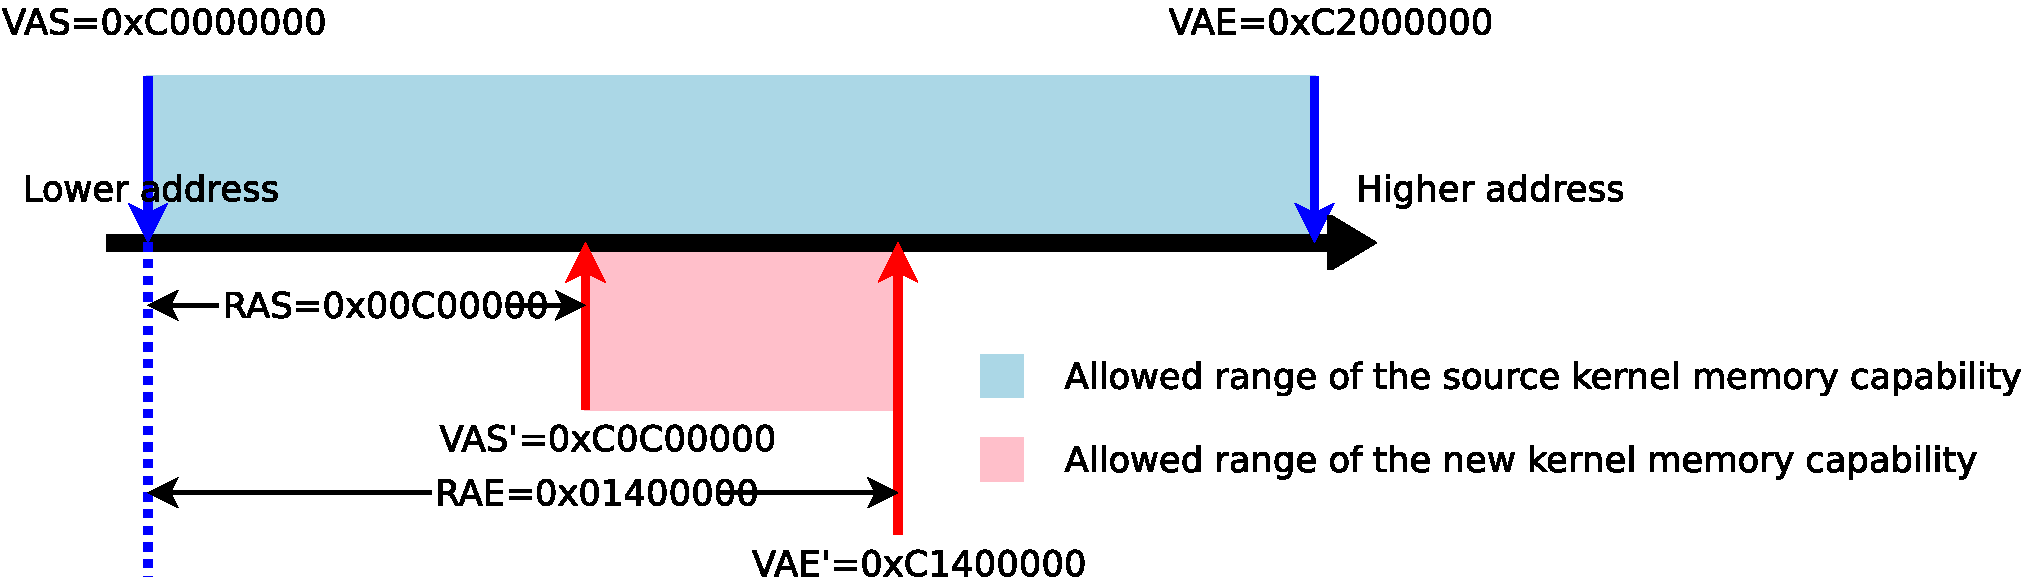
\includegraphics[width=0.72\textwidth]{Figure/image10.pdf}
    \caption{Example of Kernel Memory Capability Delegation}
    \label{fig:3-3-kernel-memory-capability-transfer-example}
\end{figure}

In addition, the upper bound value of the kernel memory capability\footnote{That is, the kernel end absolute virtual address} does not include itself. In the above example, 0xC1400000 is not included in the legal addresses operable by the new kernel memory capability; that is, the kernel memory range actually permitted is 0xC0C00000-0xC13FFFFF. The upper bound must be greater than the lower bound; otherwise, an error is returned. When passed in, both the upper bound and the lower bound have their last six bits masked off, aligning them to 64 bytes. If the kernel memory registry table is configured to use slots larger than 64 bytes, the kernel automatically rounds the passed-in lower bound up and the upper bound down to align to the slot size.

The possible return values of this system call are completely identical to those of a general RME\_SVC\_CPT\_ADD operation; please refer to \ref{subsec:2-transfer-a-capability}.

\section{Bibliography}\label{sec:3-chapter-bibliography}

\protect\phantomsection\label{cite:3-1}
{[}1{]}
Q. Wang, Y. Ren, M. Scaperoth, and G. Parmer, "Speck: A kernel for
scalable predictability," in Real-Time and Embedded Technology and
Applications Symposium (RTAS), 2015 IEEE, 2015, pp. 121-132.

\protect\phantomsection\label{cite:3-2}
{[}2{]} Emcraft Systems. uCLinux(2017).
\url{https://github.com/EmcraftSystems/linux-emcraft}

\protect\phantomsection\label{cite:3-3}
{[}3{]} G. Klein, K. Elphinstone, G. Heiser, J. Andronick, D. Cock, P.
Derrin, et al., "seL4: formal verification of an OS kernel," presented
at the Proceedings of the ACM SIGOPS 22nd symposium on Operating systems
principles, Big Sky, Montana, USA, 2009.

\protect\phantomsection\label{cite:3-4}
{[}4{]} Fiasco.OC website (2017).
\url{http://os.inf.tu-dresden.de/fiasco}
